\chapter{Validation/Case studies}\label{chap:validation}

The created tools and platform are now functional for testing problems, but they have not yet been tested in real-world scenarios. They have to be validated with real case studies in the areas of biotechnology and health where the application of these tools is relevant. This is the purpose of this chapter.

\section{The Datasets}\label{sec:datasets}

In total, 2 datasets were used as case studies and Table~\ref{tab:case_studies} provides an overview. The last column contains the dataset size with the number of negative and positive labels.

\begin{table}[ht]
	\caption{Case studies.}
	\label{tab:case_studies}
    \centering
    \begin{tabular}{lp{2cm}p{3.5cm}p{3.4cm}l}
    	\toprule
    	\textbf{Year} & \textbf{Authors} & \textbf{Title} & \textbf{Focus} & \textbf{Size (Negative/Positive)}\\\midrule
    	
    	% 2016 & \citeauthor{Nguyen2016DNANetwork} & DNA Sequence Classification by Convolutional Neural Network~\cite{Nguyen2016DNANetwork} & Predict histone profiles from \gls{DNA} sequences. & 7296/7667\\\midrule
    	
        2018 & \citeauthor{Zou2018AGenomics} & A primer on deep learning in genomics~\cite{Zou2018AGenomics} & Discovery of transcription-factor binding sites in \gls{DNA}. & 1013/987\\\midrule
        
        2020 & \citeauthor{Zhang2020DeepHE:Learning} & DeepHE~\cite{Zhang2020DeepHE:Learning} & Predicting human essential genes based on deep learning. & 12624/2010\\
        
    	\bottomrule
    \end{tabular}
\end{table}

% The first dataset used in this study, as well as in a previous work in the literature~\cite{Nguyen2016DNANetwork}, is one of the datasets published by~\citeauthor{Pokholok2005Genome-wideYeast}~\cite{Pokholok2005Genome-wideYeast}. These datasets are about \gls{DNA} sequences wrapping around histone proteins. It is a method for storing and packing lengthy \gls{DNA} sequences within the nucleus of a cell. The chosen dataset contains histones of type H3, with 7667 positive labels and 7296 negative labels and sequences with length 500. \citeauthor{Nguyen2016DNANetwork}~\cite{Nguyen2016DNANetwork} achieved 89\% accuracy in the H3 dataset in their work.

The first dataset used was derived from a study of~\citeauthor{Zou2018AGenomics}~\cite{Zou2018AGenomics}. The authors addressed an important problem in functional genomics, which is the discovery of transcription-factor binding sites in \gls{DNA}. They created a neural network capable of discovering \gls{DNA} binding motifs based on the results of a test that evaluates whether a longer \gls{DNA} sequence binds to the protein or not. The dataset has 2000 \gls{DNA} sequences of length 50, with 987 positive labels and 1013 negative labels. According to the experiments, the model achieved 98\% accuracy on the testing data.

The second used in this study was used in a research paper from~\citeauthor{Zhang2020DeepHE:Learning}. The authors tackled the issue that the majority of essential gene prediction approaches based on \gls{ML} lack the necessary ability to handle the unbalanced learning problem that is inherent in the challenge, which may be one reason impacting their performance. By combining features from sequencing data and protein-protein interaction network, the authors proposed a \gls{DL}-based approach, \textit{DeepHE}, to predict human essential genes. According to the experiment results, \textit{DeepHE} outperformed \gls{ML} models, such as \gls{SVM}, Naive Bayes, \gls{RF}, and Adaboost, achieving results of 90\% accuracy on the testing data. 

\section{Data Collection and Transformation}

The first dataset was easily accessible. The article included a link to the accompanying \textit{CSV} file containing the sequences and their labels and no further data cleaning was required. 

The second dataset was not as easily accessible. Instead of providing a \textit{CSV} file, the authors specified the names of the databases from which they got the data. They built the essential gene dataset from the \textit{DEG} database~\cite{Luo2014DEGElements}, and obtained the non-essential gene sequences from \textit{Ensembl} database~\cite{Ruffier2017EnsemblAnnotation}. The \textit{DEG} database contained 16 different human essential genes datasets, and 8256 human genes are identified as essential in at least one of the 16 datasets. However, the authors assumed that about 10\% human genes might be essential genes, and decided to build the essential gene dataset with genes contained at least in 5 datasets, resulting in 2024 sequences.

Then, for the non-essential gene dataset, the authors only stated that they obtained the sequences from \textit{Ensembl}. However, the \textit{Ensembl} database contains many different queries and options, and the authors did not specify which ones they used. This lack of information made it difficult to obtain the exact same dataset as the used on the paper. The only provided information is that they downloaded the dataset from \textit{Ensembl} and, if any of the 8256 annotated essential \textit{DEG} genes were present in the new dataset, they were deleted, resulting in 12697 sequences.

The attempt of replicating the paper's non-essential genes dataset was the following:

\begin{enumerate}
    \item The Human genes dataset was downloaded from the \textit{Ensembl} 97 release, with unspliced gene and protein coding gene type filters, which resulted in 22722 entries in a \textit{FASTA} file. Each entry is a pair of key and value, with each key being a set of 4 ids (gene stable ID, gene stable ID version, transcript stable ID, transcript stable ID version), and the value being the sequence.
    \item Similarly to the study, sequences in this dataset that also appeared in the \textit{DEG} dataset were removed, resulting in 22699 entries.
    \item It was noticed that the previous step hardly affected the dataset, but the sequences from \textit{DEG} dataset had an id (EMBL or HGNC ids) which was later found that refered to the gene stable ID of the \textit{Ensembl} dataset. All of the ids from the \textit{Ensembl} dataset that appeared in the \textit{DEG} were removed, along with the sequences associated, resulting in 15888 entries.
    \item Then, a cleaning step was performed, where sequences that repeated in the dataset or with invalid characters were removed, resulting in 15137 entries.
\end{enumerate}

As expected, the results of attempting to replicate these steps for the positive and negative datasets were not the same to those in the study. Only 2010 sequences were retrieved for the positive dataset, while 15137 sequences were obtained for the negative dataset. The size of the positive dataset is comparable to that of the study, but the negative still had a relevant discrepancy. 

However, it is important to note that the sequences did not have the same length, unlike the two first datasets. Figures~\ref{fig:deg_length} and~\ref{fig:negative}  provide a visualization of the sequences length distribution in each dataset.

\begin{figure}[htbp]
    \centering
    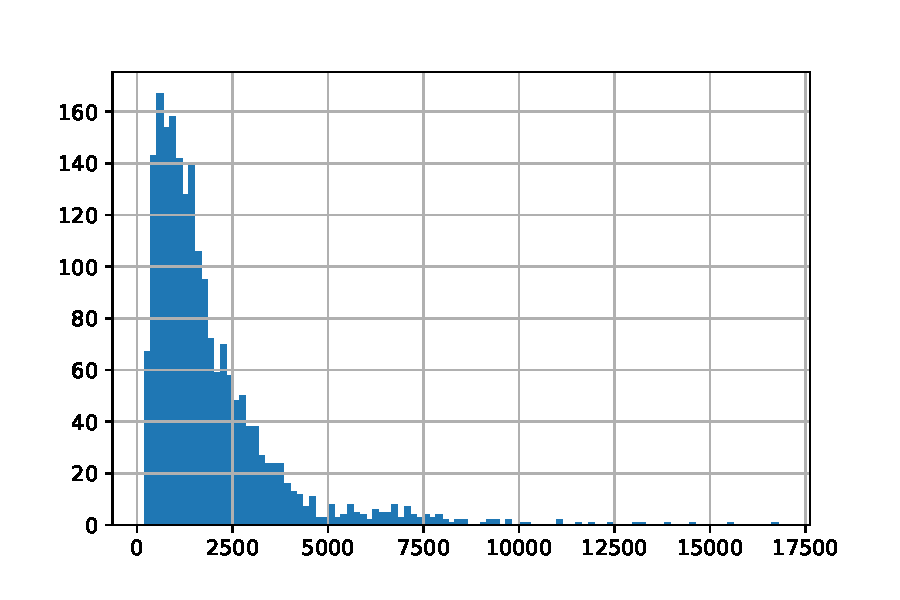
\includegraphics[width=0.7\linewidth]{positive}
    \caption{Sequence length and its occurrence in the positive dataset.}
    \label{fig:deg_length}
\end{figure}

\begin{figure}[htbp]
    \centering
    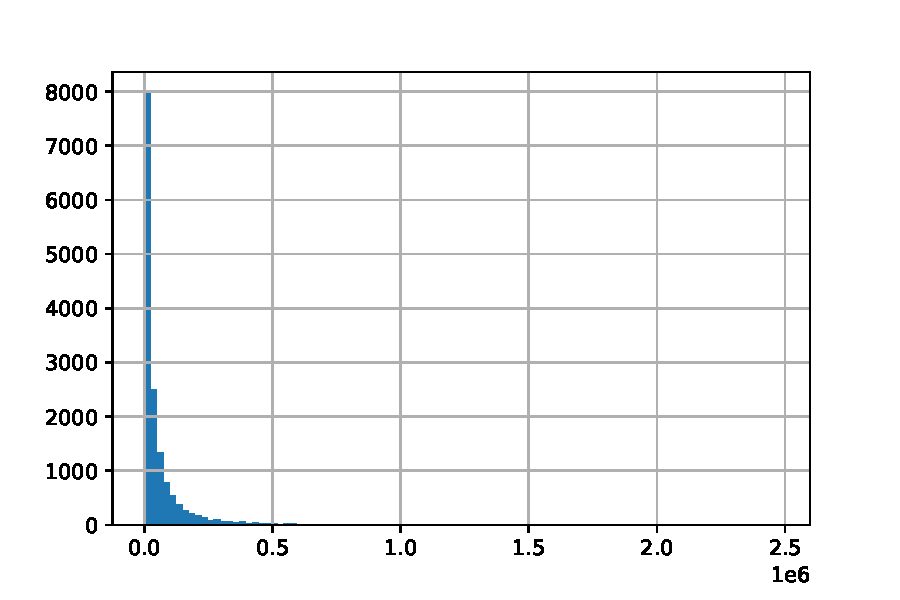
\includegraphics[width=0.7\linewidth]{negative}
    \caption{Sequence length and its occurrence in the negative dataset.}
    \label{fig:negative}
\end{figure}

A significant disparity in the length of the sequences was found in both datasets, especially in the negative one. The majority of the sequences have a length between 0 and 0.1e6. To remove some data noise, to balance the sequences length distribution and to attempt to achieve a better approximation to the size of the study's negative dataset, sequences that had length bigger than 0.1e6 were deleted, resulting in 12624 sequences. Even though the lengths of the positive dataset are not balanced either, no sequences were removed because the number of sequences was already very close to the paper's.

\begin{figure}[htbp]
    \centering
    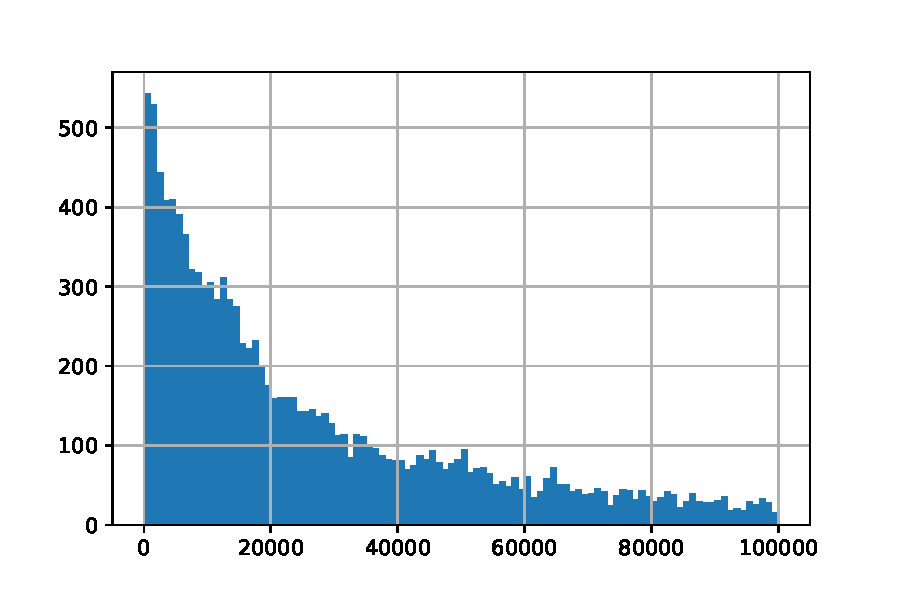
\includegraphics[width=0.7\linewidth]{negative_less_100k}
    \caption{Sequence length and its occurrence after removing sequences bigger than 0.1e6.}
    \label{fig:negative_less_100k}
\end{figure}

The final version of this dataset was 2010 positives and 12624 negatives. Even though it is not exactly the same size of the study, it was considered a satisfactory approximation.

As mentioned in Section~\ref{sec:setup}, the sequence feature vectors that will be fed into the model need to have the same input shape, regardless of whether the sequences have the same length or not. Unlike the previous datasets, this one did not have sequences with uniform length. When using descriptors, this is not relevant, since they were implemented in a way that they are not dependent on the sequence's length. However, for the encodings, a length value was required, and sequences larger than that value were trimmed, while those shorter than that value were filled with letter N's. Figures~\ref{fig:deg_length} and~\ref{fig:negative_less_100k} depict the lengths distribution in the positive and negative datasets, respectively, and it can be concluded that the lengths are significantly different between the two. Some computed statistics from the two datasets are shown below in Table~\ref{tab:stats}.

\begin{table}[ht]
	\caption{Statistics about the positive and negative datasets.}
	\label{tab:stats}
    \centering
    \begin{tabular}{llll}
    	\toprule
    	\textbf{Class} & \textbf{Smallest length} & \textbf{Biggest length} & \textbf{Mean length}\\\midrule
    	
    	Negative & 76 & 99993 & 25173\\\midrule
        Positive & 192 & 16791 & 1903\\
        
    	\bottomrule
    \end{tabular}
\end{table}

One approach would be setting the length to the maximum value, avoiding the cut of sequences. Table~\ref{tab:stats} reveals, however, that it would add a significant amount of data noise to the dataset, since the largest value (99993) is far from the mean length of both datasets. The length value was chosen to 2000 in order to reduce the number of N's added to sequences. This way, the positive sequences did not suffer much modifications, and most of the negative ones were trimmed. In their investigation, the authors skipped this step since they extracted features from sequences (descriptors) and did not do any encoding calculations.

\section{Optimal Class Weight}

Unlike the first dataset, the second one is greatly unbalanced, with 2010 positive labels and 12624 negative ones. This can be an obstacle for the training of the model, as it is more likely to predict the negative class. To address the uneven data distributions between the two classes, class weights were used to impose a heavier penalty when misclassifying an instance in the minority class, which is the class of essential genes. Experiments were conducted to determine the ideal weight assigned to each class, and can be found below in Table~\ref{tab:weights}.

As the objective is to discover the optimal class weight to train the models for the essential genes dataset, it would be pointless to test all possible combinations of feature extractions techniques and models, as doing so would create an enormous number of possibilities. So, there had to be a selection of feature extractions methods as well as models to test the different weight classes. For feature extraction, only descriptors and one-hot encoding were selected, and for models, the \gls{MLP}, \gls{CNN}, \gls{LSTM}, and \gls{GRU} were picked, as the remaining models are built using one or more of these four.

\begin{table}[ht]
	\caption{Results of different weights in the essential genes dataset.}
	\label{tab:weights}
    \centering
    \begin{tabular}{lllllll}
    	\toprule
    	\textbf{Model} & \textbf{Feature Extraction} & \textbf{Weights} & \textbf{Accuracy}  & \textbf{MCC} & \textbf{Confusion Matrix}\\\midrule
    	
    	MLP & Descriptor & 1:1 & 0.978 & 0.911 & 
    	$\begin{bmatrix}
            2485 & 40\\ 
            23 & 379
        \end{bmatrix}$
        \\
        
        MLP & Descriptor & 1:2 & 0.979 & 0.915 & 
    	$\begin{bmatrix}
            2482 & 43\\ 
            18 & 384
        \end{bmatrix}$
        \\
        
        \textbf{MLP} & \textbf{Descriptor} & \textbf{1:3} & \textbf{0.980} & \textbf{0.918} & 
    	$\begin{bmatrix}
            2487 & 38\\ 
            20 & 382
        \end{bmatrix}$
        \\
        
        MLP & Descriptor & 1:4 & 0.978 & 0.913 & 
    	$\begin{bmatrix}
            2477 & 48\\ 
            15 & 387
        \end{bmatrix}$
        \\\midrule
        
        \textbf{CNN} & \textbf{One-Hot} & \textbf{1:1} & \textbf{0.964} & \textbf{0.845} & 
    	$\begin{bmatrix}
            2478 & 47\\ 
            59 & 343
        \end{bmatrix}$
        \\
        
        CNN & One-Hot & 1:2 & 0.956 & 0.815 & 
    	$\begin{bmatrix}
            2459 & 66\\ 
            63 & 339
        \end{bmatrix}$
        \\
        
        CNN & One-Hot & 1:3 & 0.957 & 0.823 & 
    	$\begin{bmatrix}
            2454 & 71\\ 
            54 & 348
        \end{bmatrix}$
        \\
        
        CNN & One-Hot & 1:4 & 0.945 & 0.785 & 
    	$\begin{bmatrix}
            2413 & 112\\ 
            49 & 353
        \end{bmatrix}$
        \\\midrule
        
        LSTM & One-Hot & 1:1 & 0.974 & 0.899 & 
    	$\begin{bmatrix}
            2459 & 66\\ 
            10 & 392
        \end{bmatrix}$
        \\
        
        \textbf{LSTM} & \textbf{One-Hot} & \textbf{1:2} & \textbf{0.978} & \textbf{0.907} & 
    	$\begin{bmatrix}
            2490 & 35\\ 
            30 & 372
        \end{bmatrix}$
        \\
        
        LSTM & One-Hot & 1:3 & 0.972 & 0.890 & 
    	$\begin{bmatrix}
            2459 & 66\\ 
            16 & 386
        \end{bmatrix}$
        \\
        
        LSTM & One-Hot & 1:4 & 0.976 & 0.908 & 
    	$\begin{bmatrix}
            2465 & 60\\ 
            9 & 393
        \end{bmatrix}$
        \\\midrule
        
        \textbf{GRU} & \textbf{One-Hot} & \textbf{1:1} & \textbf{0.982} & \textbf{0.925} & 
    	$\begin{bmatrix}
            2497 & 28\\ 
            24 & 378
        \end{bmatrix}$
        \\
        
        GRU & One-Hot & 1:2 & 0.979 & 0.913 & 
    	$\begin{bmatrix}
            2490 & 35\\ 
            26 & 376
        \end{bmatrix}$
        \\
        
        GRU & One-Hot & 1:3 & 0.980 & 0.916 & 
    	$\begin{bmatrix}
            2485 & 40\\ 
            20 & 382
        \end{bmatrix}$
        \\
        
        GRU & One-Hot & 1:4 & 0.981 & 0.920 & 
    	$\begin{bmatrix}
            2484 & 41\\ 
            16 & 386
        \end{bmatrix}$
        \\
        
    	\bottomrule
    \end{tabular}
\end{table}

By reviewing the data in Table~\ref{tab:weights}, one could conclude that class weights have a minimal effect on the performance of each model. In fact, in certain models, the best results can be achieved without any class weight distribution at all. Due to the robustness of the models, it is reasonable to infer that the class imbalance is not a significant concern. In addition, it can be inferred that, with the exception of the \gls{CNN} model, every other model achieves roughly the same level of accuracy regardless of the weight distribution, confirming the belief that the class imbalance is not a significant issue.

Therefore, no weight class distribution was selected for training the remaining feature extraction techniques and model combinations in the essential genes dataset, since it was the best performing in half of the models.


\section{Results}\label{lab:results}

To acquire the best possible results, it was necessary to test every combination of feature extraction - model - dataset. There are a total of four types of feature extraction techniques, ten distinct models, and two datasets. This means that, so far, $4*10*2 = 80$ possibilities would need testing. 

However, one of the feature extraction methods, the k-mer one-hot encoding, receives a parameter \textit{k} defined by the user. The number of possibilities will rapidly increase since every value of $k$ would have to be tested, and $0 < k < L$, where $L$ is the length of the sequence. Given a sequence with length 2000 (sequences' length in the essential genes dataset), the number of possibilities that would need testing would be $(3+2000) * 10 * 3 = 60090$. Due to the practical impossibility of testing this number of possibilities, a maximum value for $k$ had to be established. It is also important to mention that the bigger the value of $k$, the larger the feature vector will be. With $k = 10$, every word of 10 letters (AAAAAAAAAA, AAAAAAAAAT, ..., NNNNNNNNNN) had to be calculated and assigned a unique array to represent it. This would result in 9765625 possible combinations, with each one assigned to an array of also $5^{10} = 9765625$ elements (containing exclusively zeros with the exception of a single 1 at a single position in the array). Then, the sequence had to be separated into $L-k+1 = 2000 - 10 + 1 = 1991$ 10-mers and assign the respective array of 9765625 elements, resulting in a vector size of $1991 * 9765625 = 1.94e10$.

The time necessary to create this encoding in addition to the time required for the model to process all of this input and train with it makes large values of $k$ impractical. This was taken into account while determining the maximum value of $k$, so that this value would be related with the maximum acceptable amount of time to wait for classification results. Some experiments to find the maximum value of $k$ were performed in the essential genes dataset, which is the dataset with the largest sequences, and the \gls{CNN} model, which is the \gls{DL} model with the fastest train times. They can be found below in Table~\ref{tab:stats_kmer}.

\begin{table}[ht]
	\caption{Statistics about the k-mer one-hot encoding on the essential genes dataset using the CNN model.}
	\label{tab:stats_kmer}
    \centering
    \begin{tabular}{lll}
    	\toprule
    	\textbf{K} & \textbf{Feature Vector Size of a single sequence} & \textbf{Time to train (min)}\\\midrule
    	
    	1 & $(2000 - 1 + 1) * 5^{1} = 10\;000$ & 3 \\\midrule
        2 & $(2000 - 2 + 1) * 5^{2} = 49\;975$ & 6\\\midrule
        3 & $(2000 - 3 + 1) * 5^{3} = 249\;750$ & 27\\\midrule
        4 & $(2000 - 4 + 1) * 5^{4} = 1\;248\;125$ & Out of memory\\
        
    	\bottomrule
    \end{tabular}
\end{table}

As anticipated, both the size of the feature vector and the training time for the model increase exponentially with the value of $k$. In fact, the vector size is so large that it was not possible to train the model for $k=4$ due to limited computation resources, especifically memory. Considering the results of Table~\ref{tab:stats_kmer}, it was determined that the maximum value of k would be 3.

So, at this point, there are 5 possible feature extraction methods (descriptors, one-hot, chemical, k-mer one-hot with $k = 2$, and k-mer one-hot with $k = 3$), 10 different models and 2 datasets, resulting in 100 possibilities that would need testing. However, some of these combinations are incompatible (some models only accept encodings and vice-versa). Therefore, 74 combinations were examined, and the results are shown below in Table~\ref{tab:primer_results} and in Table~\ref{tab:eg_results}. It also worth mentioning that these results were obtained using the cross entropy loss function, which is the default loss function to use for binary classification problems~\cite{BrownleeHowNetworks}, and the Adam optimizer, which is one of the most popular optimizers and was the one used in both case studies.

\begin{longtable}{llllll}
	\caption{Results on Primer dataset.}
	\label{tab:primer_results}
    \endfirsthead
    \endhead
    
	\textbf{Model} & \textbf{Feature Extraction} & \textbf{Accuracy}  & \textbf{MCC} & \textbf{Confusion Matrix}\\\midrule
	
	MLP & Descriptor & 0.958 & 0.917 & 
	$\begin{bmatrix}
        188 & 15\\ 
        2 & 195
    \end{bmatrix}$
    \\\midrule

    %%%%%%%%%%%%%%%%%%%%%%%%%%%%%%%%%%%%%%%%%%%%%%

    CNN & One-Hot & 0.990 & 0.980 & 
	$\begin{bmatrix}
        199 & 4\\ 
        0 & 197
    \end{bmatrix}$
    \\

    CNN & Chemical & 0.988 & 0.975 & 
	$\begin{bmatrix}
        199 & 4\\ 
        1 & 196
    \end{bmatrix}$
    \\

    CNN & 2-mer one-hot & 0.985 & 0.970 & 
	$\begin{bmatrix}
        197 & 6\\ 
        0 & 197
    \end{bmatrix}$
    \\

    CNN & 3-mer one-hot & 0.995 & 0.990 & 
	$\begin{bmatrix}
        201 & 2\\ 
        0 & 197
    \end{bmatrix}$
    \\\midrule

    %%%%%%%%%%%%%%%%%%%%%%%%%%%%%%%%%%%%%%%%%%%%%%

    LSTM & One-hot & 0.998 & 0.995 & 
	$\begin{bmatrix}
        202 & 1\\ 
        0 & 197
    \end{bmatrix}$
    \\

    LSTM & Chemical & 0.998 & 0.995 & 
	$\begin{bmatrix}
        202 & 1\\ 
        0 & 197
    \end{bmatrix}$
    \\

    LSTM & 2-mer one-hot & 1 & 1 & 
	$\begin{bmatrix}
        203 & 0\\ 
        0 & 197
    \end{bmatrix}$
    \\

    LSTM & 3-mer one-hot & 1 & 1 & 
	$\begin{bmatrix}
        203 & 0\\ 
        0 & 197
    \end{bmatrix}$
    \\\midrule
    
    %%%%%%%%%%%%%%%%%%%%%%%%%%%%%%%%%%%%%%%%%%%%%%

    BiLSTM & One-hot & 1 & 1 &
    $\begin{bmatrix}
        203 & 0\\ 
        0 & 197
    \end{bmatrix}$
    \\

    BiLSTM & Chemical & 1 & 1 &
    $\begin{bmatrix}
        203 & 0\\ 
        0 & 197
    \end{bmatrix}$
    \\

    BiLSTM & 2-mer one-hot & 1 & 1 &
    $\begin{bmatrix}
        203 & 0\\ 
        0 & 197
    \end{bmatrix}$
    \\

    BiLSTM & 3-mer one-hot & 1 & 1 &
    $\begin{bmatrix}
        203 & 0\\ 
        0 & 197
    \end{bmatrix}$
    \\\midrule
            
    %%%%%%%%%%%%%%%%%%%%%%%%%%%%%%%%%%%%%%%%%%%%%%

    GRU & One-hot & 1 & 1 &
    $\begin{bmatrix}
        203 & 0\\ 
        0 & 197
    \end{bmatrix}$
    \\

    GRU & Chemical & 1 & 1 &
    $\begin{bmatrix}
        203 & 0\\ 
        0 & 197
    \end{bmatrix}$
    \\

    GRU & 2-mer one-hot & 1 & 1 &
    $\begin{bmatrix}
        203 & 0\\ 
        0 & 197
    \end{bmatrix}$
    \\

    GRU & 3-mer one-hot & 0.995 & 0.990 &
    $\begin{bmatrix}
        201 & 2\\ 
        0 & 197
    \end{bmatrix}$
    \\\midrule

    %%%%%%%%%%%%%%%%%%%%%%%%%%%%%%%%%%%%%%%%%%%%%%

    Bi-GRU & One-hot & 0.998 & 0.995 &
    $\begin{bmatrix}
        202 & 1\\ 
        0 & 197
    \end{bmatrix}$
    \\

    Bi-GRU & Chemical & 1 & 1 &
    $\begin{bmatrix}
        203 & 0\\ 
        0 & 197
    \end{bmatrix}$
    \\

    Bi-GRU & 2-mer one-hot & 0.993 & 0.985 &
    $\begin{bmatrix}
        200 & 3\\ 
        0 & 197
    \end{bmatrix}$
    \\

    Bi-GRU & 3-mer one-hot & 1 & 1 &
    $\begin{bmatrix}
        203 & 0\\ 
        0 & 197
    \end{bmatrix}$
    \\\midrule

    %%%%%%%%%%%%%%%%%%%%%%%%%%%%%%%%%%%%%%%%%%%%%%

    CNN-LSTM & One-hot & 0.978 & 0.956 &
    $\begin{bmatrix}
        194 & 9\\ 
        0 & 197
    \end{bmatrix}$
    \\

    CNN-LSTM & Chemical & 0.985 & 0.970 &
    $\begin{bmatrix}
        197 & 6\\ 
        0 & 197
    \end{bmatrix}$
    \\

    CNN-LSTM & 2-mer one-hot & 0.990 & 0.980 &
    $\begin{bmatrix}
        199 & 4\\ 
        0 & 197
    \end{bmatrix}$
    \\

    CNN-LSTM & 3-mer one-hot & 0.998 & 0.995 &
    $\begin{bmatrix}
        202 & 1\\ 
        0 & 197
    \end{bmatrix}$
    \\\midrule

    %%%%%%%%%%%%%%%%%%%%%%%%%%%%%%%%%%%%%%%%%%%%%%

    CNN-BiLSTM & One-hot & 0.988 & 0.975 &
    $\begin{bmatrix}
        199 & 4\\ 
        1 & 196
    \end{bmatrix}$
    \\

    CNN-BiLSTM & Chemical & 0.960 & 0.923 &
    $\begin{bmatrix}
        187 & 16\\
        0 & 197
    \end{bmatrix}$
    \\

    CNN-BiLSTM & 2-mer one-hot & 0.995 & 0.990 &
    $\begin{bmatrix}
        201 & 2\\ 
        0 & 197
    \end{bmatrix}$
    \\

    CNN-BiLSTM & 3-mer one-hot & 0.998 & 0.995 &
    $\begin{bmatrix}
        202 & 1\\ 
        0 & 197
    \end{bmatrix}$
    \\\midrule

    %%%%%%%%%%%%%%%%%%%%%%%%%%%%%%%%%%%%%%%%%%%%%%

    CNN-GRU & One-hot & 0.985 & 0.970 &
    $\begin{bmatrix}
        197 & 6\\ 
        0 & 197
    \end{bmatrix}$
    \\

    CNN-GRU & Chemical & 0.995 & 0.990 &
    $\begin{bmatrix}
        201 & 2\\ 
        0 & 197
    \end{bmatrix}$
    \\

    CNN-GRU & 2-mer one-hot & 0.995 & 0.990 &
    $\begin{bmatrix}
        201 & 2\\ 
        0 & 197
    \end{bmatrix}$
    \\

    CNN-GRU & 3-mer one-hot & 0.985 & 0.970 &
    $\begin{bmatrix}
        202 & 1\\ 
        5 & 192
    \end{bmatrix}$
    \\\midrule

    %%%%%%%%%%%%%%%%%%%%%%%%%%%%%%%%%%%%%%%%%%%%%%

    CNN-BiGRU & One-hot & 0.993 & 0.985 &
    $\begin{bmatrix}
        200 & 3\\ 
        0 & 197
    \end{bmatrix}$
    \\

    CNN-BiGRU & Chemical & 0.990 & 0.980 &
    $\begin{bmatrix}
        199 & 4\\ 
        0 & 197
    \end{bmatrix}$
    \\

    CNN-BiGRU & 2-mer one-hot & 0.995 & 0.990 &
    $\begin{bmatrix}
        201 & 2\\ 
        0 & 197
    \end{bmatrix}$
    \\

    CNN-BiGRU & 3-mer one-hot & 0.998 & 0.995 &
    $\begin{bmatrix}
        202 & 1\\ 
        0 & 197
    \end{bmatrix}$
    \\
    
	\bottomrule
\end{longtable}


\begin{longtable}{llllll}
	\caption{Results on Essential Genes dataset.}
	\label{tab:eg_results}
    \endfirsthead
    \endhead
    
	\textbf{Model} & \textbf{Feature Extraction} & \textbf{Accuracy}  & \textbf{MCC} & \textbf{Confusion Matrix}\\\midrule
	
	MLP & Descriptor & 0.978 & 0.911 & 
	$\begin{bmatrix}
        2485 & 40\\ 
        23 & 379
    \end{bmatrix}$
    \\\midrule

    %%%%%%%%%%%%%%%%%%%%%%%%%%%%%%%%%%%%%%%%%%%%%%

    CNN & One-Hot & 0.964 & 0.845 &
	$\begin{bmatrix}
        2478 & 47\\ 
        59 & 343
    \end{bmatrix}$
    \\

    CNN & Chemical & 0.950 & 0.782 &
	$\begin{bmatrix}
        2476 & 49\\ 
        96 & 306
    \end{bmatrix}$
    \\

    CNN & 2-mer one-hot & 0.965 & 0.855 & 
	$\begin{bmatrix}
        2462 & 63\\ 
        40 & 362
    \end{bmatrix}$
    \\

    CNN & 3-mer one-hot & 0.978 & 0.912 & 
	$\begin{bmatrix}
        2483 & 42\\ 
        21 & 381
    \end{bmatrix}$
    \\\midrule

    %%%%%%%%%%%%%%%%%%%%%%%%%%%%%%%%%%%%%%%%%%%%%%

    LSTM & One-hot & 0.980 & 0.916 & 
	$\begin{bmatrix}
        2489 & 36\\ 
        23 & 379
    \end{bmatrix}$
    \\

    LSTM & Chemical & ??? & ??? & 
	$\begin{bmatrix}
        ??? & ???\\ 
        ??? & ???
    \end{bmatrix}$
    \\

    LSTM & 2-mer one-hot & ??? & ??? & 
	$\begin{bmatrix}
        ??? & ???\\ 
        ??? & ???
    \end{bmatrix}$
    \\

    LSTM & 3-mer one-hot & ??? & ??? & 
	$\begin{bmatrix}
        ??? & ???\\ 
        ??? & ???
    \end{bmatrix}$
    \\\midrule
    
    %%%%%%%%%%%%%%%%%%%%%%%%%%%%%%%%%%%%%%%%%%%%%%

    BiLSTM & One-hot & ??? & ??? &
    $\begin{bmatrix}
        ??? & ???\\ 
        ??? & ???
    \end{bmatrix}$
    \\

    BiLSTM & Chemical & ??? & ??? &
    $\begin{bmatrix}
        ??? & ???\\ 
        ??? & ???
    \end{bmatrix}$
    \\

    BiLSTM & 2-mer one-hot & ??? & ??? &
    $\begin{bmatrix}
        ??? & ???\\ 
        ??? & ???
    \end{bmatrix}$
    \\

    BiLSTM & 3-mer one-hot & ??? & ??? &
    $\begin{bmatrix}
        ??? & ???\\ 
        ??? & ???
    \end{bmatrix}$
    \\\midrule
            
    %%%%%%%%%%%%%%%%%%%%%%%%%%%%%%%%%%%%%%%%%%%%%%

    GRU & One-hot & 0.977 & 0.900 &
    $\begin{bmatrix}
        2506 & 19\\ 
        49 & 353
    \end{bmatrix}$
    \\

    GRU & Chemical & ??? & ??? &
    $\begin{bmatrix}
        ??? & ???\\ 
        ??? & ???
    \end{bmatrix}$
    \\

    GRU & 2-mer one-hot & ??? & ??? &
    $\begin{bmatrix}
        ??? & ???\\ 
        ??? & ???
    \end{bmatrix}$
    \\

    GRU & 3-mer one-hot & ??? & ??? &
    $\begin{bmatrix}
        ??? & ???\\ 
        ??? & ???
    \end{bmatrix}$
    \\\midrule

    %%%%%%%%%%%%%%%%%%%%%%%%%%%%%%%%%%%%%%%%%%%%%%

    Bi-GRU & One-hot & ??? & ??? &
    $\begin{bmatrix}
        ??? & ???\\ 
        ??? & ???
    \end{bmatrix}$
    \\

    Bi-GRU & Chemical & ??? & ??? &
    $\begin{bmatrix}
        ??? & ???\\ 
        ??? & ???
    \end{bmatrix}$
    \\

    Bi-GRU & 2-mer one-hot & ??? & ??? &
    $\begin{bmatrix}
        ??? & ???\\ 
        ??? & ???
    \end{bmatrix}$
    \\

    Bi-GRU & 3-mer one-hot & ??? & ??? &
    $\begin{bmatrix}
        ??? & ???\\ 
        ??? & ???
    \end{bmatrix}$
    \\\midrule

    %%%%%%%%%%%%%%%%%%%%%%%%%%%%%%%%%%%%%%%%%%%%%%

    CNN-LSTM & One-hot & 0.958 & 0.821 &
    $\begin{bmatrix}
        2468 & 57\\
        66 & 336
    \end{bmatrix}$
    \\

    CNN-LSTM & Chemical & 0.942 & 0.742 &
    $\begin{bmatrix}
        2465 & 60\\ 
        111 & 291
    \end{bmatrix}$
    \\

    CNN-LSTM & 2-mer one-hot & 0.971 & 0.878 &
    $\begin{bmatrix}
        2482 & 43\\ 
        42 & 360
    \end{bmatrix}$
    \\

    CNN-LSTM & 3-mer one-hot & 0.973 & 0.885 &
    $\begin{bmatrix}
        2489 & 36\\ 
        43 & 359
    \end{bmatrix}$
    \\\midrule

    %%%%%%%%%%%%%%%%%%%%%%%%%%%%%%%%%%%%%%%%%%%%%%

    CNN-BiLSTM & One-hot & 0.960 & 0.836 &
    $\begin{bmatrix}
        2454 & 71\\ 
        46 & 356
    \end{bmatrix}$
    \\

    CNN-BiLSTM & Chemical & 0.936 & 0.713 &
    $\begin{bmatrix}
        2473 & 52\\
        134 & 268
    \end{bmatrix}$
    \\

    CNN-BiLSTM & 2-mer one-hot & 0.967 & 0.869 &
    $\begin{bmatrix}
        2456 & 69\\ 
        27 & 375
    \end{bmatrix}$
    \\

    CNN-BiLSTM & 3-mer one-hot & 0.976 & 0.904 &
    $\begin{bmatrix}
        2476 & 49\\ 
        20 & 382
    \end{bmatrix}$
    \\\midrule

    %%%%%%%%%%%%%%%%%%%%%%%%%%%%%%%%%%%%%%%%%%%%%%

    CNN-GRU & One-hot & 0.963 & 0.842 &
    $\begin{bmatrix}
        2474 & 51\\ 
        58 & 344
    \end{bmatrix}$
    \\

    CNN-GRU & Chemical & 0.943 & 0.744 &
    $\begin{bmatrix}
        2473 & 52\\ 
        116 & 286
    \end{bmatrix}$
    \\

    CNN-GRU & 2-mer one-hot & 0.970 & 0.874 &
    $\begin{bmatrix}
        2484 & 41\\ 
        46 & 356
    \end{bmatrix}$
    \\

    CNN-GRU & 3-mer one-hot & 0.978 & 0.911 &
    $\begin{bmatrix}
        2486 & 39\\ 
        24 & 378
    \end{bmatrix}$
    \\\midrule

    %%%%%%%%%%%%%%%%%%%%%%%%%%%%%%%%%%%%%%%%%%%%%%

    CNN-BiGRU & One-hot & 0.962 & 0.837 &
    $\begin{bmatrix}
        2475 & 50\\ 
        62 & 340
    \end{bmatrix}$
    \\

    CNN-BiGRU & Chemical & 0.946 & 0.778 &
    $\begin{bmatrix}
        2434 & 91\\ 
        67 & 335
    \end{bmatrix}$
    \\

    CNN-BiGRU & 2-mer one-hot & 0.971 & 0.880 &
    $\begin{bmatrix}
        2475 & 50\\ 
        35 & 367
    \end{bmatrix}$
    \\

    CNN-BiGRU & 3-mer one-hot & 0.977 & 0.908 &
    $\begin{bmatrix}
        2480 & 45\\ 
        21 & 381
    \end{bmatrix}$
    \\
    
	\bottomrule
\end{longtable}


Analyzing both tables, it can be concluded that all feature extraction methods and models performed well in both datasets. The results in the Primer dataset are better than the Essential Genes ones, which is expected since the results from both studies also show that the Primer dataset is easier to classify than the Essential Genes one (the authors from the Primer study achieved 98\% accuracy and the authors from the Essential Genes study achieved 90\% accuracy). The results obtained outperformed the results from both studies, achieving 100\% accuracy on the Primer dataset using \gls{LSTM}, Bi-LSTM, \gls{GRU} and Bi-GRU models, and 98\% accuracy on the Essential Genes dataset using ??? combination. 

These results show that \gls{RNN} (\gls{LSTM}, \gls{GRU}, and their variations) models are the best choice for this problem, since they achieved the best results in both datasets. \gls{RNN} models are well-known for their capacity to process sequential data, which is most likely why these models produced the best results.

\section{Results Reproducibility}

A machine learning pipeline has several nondeterministic stages. For instance, the training and testing sets resulting from data splitting are very likely to change across runs. This is problematic since it makes it hard to replicate results.

However, this problem is easily tackled by using the random seed that libraries like TensorFlow and PyTorch provide. By adjusting the random seed value, it is possible to assure that random numbers are created consistently across runs. This concept may seem counterintuitive at first, since one could believe that adjusting the random seed would manipulate the algorithm's randomness. This, however, is not true. The random seed is used to guarantee that the same random numbers are produced every time, and if the random seed value is altered, so will the random numbers. This is a highly helpful feature that can help in reproducing the results, and it is a common practice in machine learning.

This line of thought can raise the question of how to choose the random seed value for optimal results. The answer to this question is that there is no single answer. The random seed value must be initially set and it is common practice to experiment with various values to see which one works best. It is, however, expected that the random seed value will not have a significant impact on the results and that the results will be similar across different values.

In this study, three different random seed values were used: 24, 42, and 2022. The results from the previous section were obtained using the random seed value of ?????. To see if the results are consistent across different random seed values, the same experiment was repeated using the other two random seed values, but only using the MLP and CNN models to reduce the number of experiments as they are already a good indicator of the consistency of the results. The results are shown in Table ??????.

% meter aqui tabela

By analyzing Table ???, it is possible to deduce that the results obtained with the other two random seed values were quite comparable to those obtained with random seed value ?????. This is a good indication that the random seed value does not have a significant impact on the results.